\documentclass[10pt,executivepaper]{article}
\usepackage[utf8]{inputenc}
\usepackage[spanish]{babel}
\usepackage{amsmath}
\usepackage{amsfonts}
\usepackage{amssymb}
\usepackage{graphics}
\usepackage{graphicx}
\usepackage[left=2cm,right=2cm,top=2cm,bottom=2cm]{geometry}
\usepackage{imakeidx}
\makeindex[columns=3, title=Alphabetical Index, intoc]
\usepackage{listings}
\usepackage{xcolor}
\usepackage{multicol}
\usepackage{changepage}
\usepackage{float}
\usepackage{cite}
\usepackage{url}
\usepackage{pdflscape}
\usepackage{listingsutf8}

\definecolor{codegreen}{rgb}{0,0.6,0}
\definecolor{codegray}{rgb}{0.5,0.5,0.5}
\definecolor{codepurple}{rgb}{0.58,0,0.82}
\definecolor{backcolour}{rgb}{0.95,0.95,0.92}

\lstdefinestyle{mystyle}{
    backgroundcolor=\color{backcolour},
    commentstyle=\color{codegreen},
    keywordstyle=\color{magenta},
    numberstyle=\tiny\color{codegray},
    stringstyle=\color{codepurple},
    basicstyle=\ttfamily\footnotesize,
    breakatwhitespace=false,
    breaklines=true,
    captionpos=b,
    keepspaces=true,
    numbers=left,
    numbersep=5pt,
    showspaces=false,
    showstringspaces=false,
    showtabs=false,
    tabsize=3,
    inputencoding=utf8,
    extendedchars=true,
    literate={á}{{\'a}}1 {ñ}{{\~n}}1 {é}{{\'e}}1,
}

\def\fillandplacepagenumber{%
 \par\pagestyle{empty}%
 \vbox to 0pt{\vss}\vfill
 \vbox to 0pt{\baselineskip0pt
   \hbox to\linewidth{\hss}%
   \baselineskip\footskip
   \hbox to\linewidth{%
     \hfil\thepage\hfil}\vss}}


\lstset{style=mystyle}

\title{Actividad: Creación de la imagen de una máquina virtual y creación de máquinas virtuales a partir de la imagen}

\author{Instituto Politécnico Nacional\\Escuela Superior de Computo\\Desarrollo de Sistemas Distribuidos\\Adrian González Pardo\\4CV1\\21/01}
\date{\today}
\newcommand\tab[1][1cm]{\hspace*{#1}}

\begin{document}
% Portada
%encabezado
\begin{minipage}{0.4\textwidth}
	\begin{flushleft}
		
\includegraphics[scale = 0.05]{logoescom.png}
	\end{flushleft}
\end{minipage}
\begin{minipage}{0.51\textwidth}
	\begin{flushright}
		
\includegraphics[scale = 0.055]{logoipn.png}
	\end{flushright}
\end{minipage}
\begin{center}
	\par\vspace{0.5cm}{
	\huge\textbf{Instituto Politécnico Nacional \\*[0.20cm] Escuela Superior de Cómputo}}
\par\vspace{1cm}{
	\large\textbf{Desarrollo de Sistemas Distribuidos\\Actividad: Creación de la imagen de una máquina virtual y creación de máquinas virtuales a partir de la imagen\\Curso impartido por el profesor: Pineda Guerrero Carlos\\Grupo: 4CV1\\21/01\\Alumno: Adrian González Pardo\\}
}
\par\vspace{1cm}{
	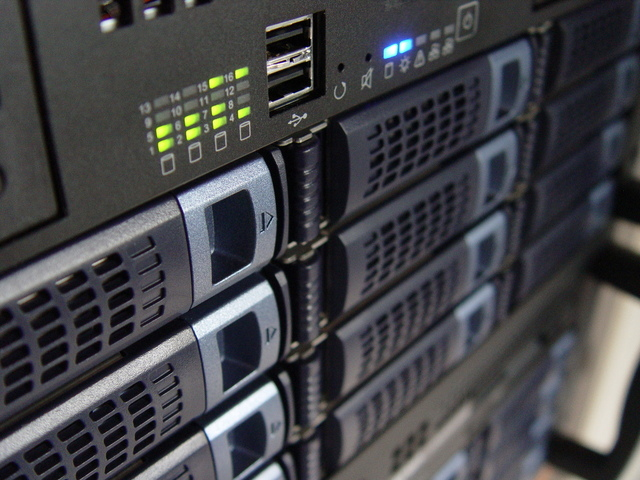
\includegraphics[scale=0.5]{servers.jpg}
}
\par\vspace{2cm}{
	Ultima fecha modificado: \today
}
\end{center}

% Indice
\clearpage
\section{Desarrollo}
Para esta practica se solicito el que ya existiera una VM creada previamente la cual puede crearse siguiendo los pasos de las practicas anteriores sin necesidad de cambiar o modificar puertos TCP, para alguna aplicación, únicamente es necesario tener la VM creada y proceder a realizar lo siguiente:
\begin{enumerate}
  \item Crear la imagen de la máquina virtual
  \item Crear una máquina virtual a partir de la imagen creada
\end{enumerate}
Entonces comenzaremos
\subsection{Crear la imagen de la máquina virtual}
Para comenzar esto podremos hacer uso de la aplicación que contenga un cliente de SSH como Putty, o por si te gusta evitar descargar una app externa tanto en Windows, Linux y hasta en MacOS es posible encontrar un cliente SSH preinstalado o que se puede instalar de forma rápida, para Windows esta PowerShell, Linux y MacOS puede encontrarse OpenSSH, una vez mencionado esto continuemos, inicialmente debemos conectarnos a la VM.\\
\begin{center}
  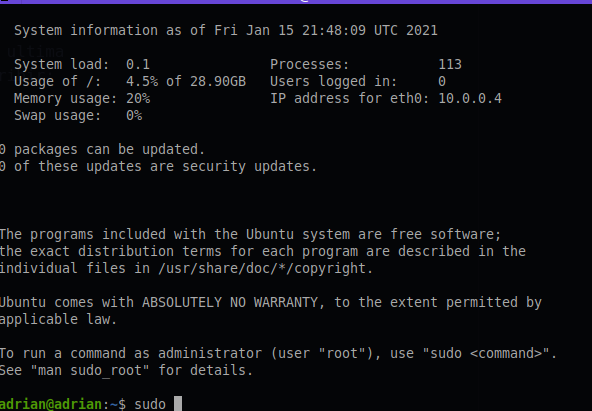
\includegraphics[scale=0.5]{imgs/1.png}\\
  \textit{Figura 1: Conexión a la VM}
\end{center}
Los primeros pasos a seguir es escribir lo siguiente en nuestra terminal:
\lstinputlisting[language=Bash]{init.sh}
\clearpage
Con ello probaremos a escribir la primer comando y obtendremos lo siguiente:
\begin{center}
  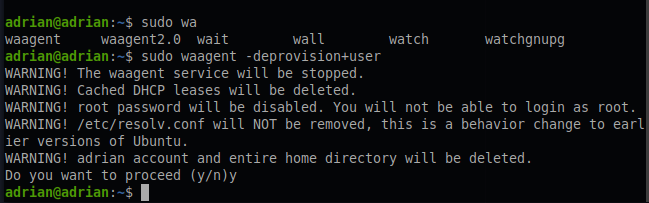
\includegraphics[scale=0.5]{imgs/2.png}\\
  \textit{Figura 2: Ejecución del primer comando}
\end{center}
Posteriormente en el menú de azure procederemos a hacer lo siguiente:
\begin{enumerate}
  \item Primeramente seleccionar la opción de captura
  \item Marcar la casilla de Eliminar automáticamente esta máquina virtual después de crear la imagen
  \item Ingresar el nombre de la VM a capturar en el apartado de definición de la imagen destino, (Primero dar en crear nuevo) y después ingresar una versión de 2 puntos ejemplo: $\#.\#.\#$, y presionar en crear recurso
  \item Finalmente esperar a que se complete el trabajo
\end{enumerate}

\begin{center}
  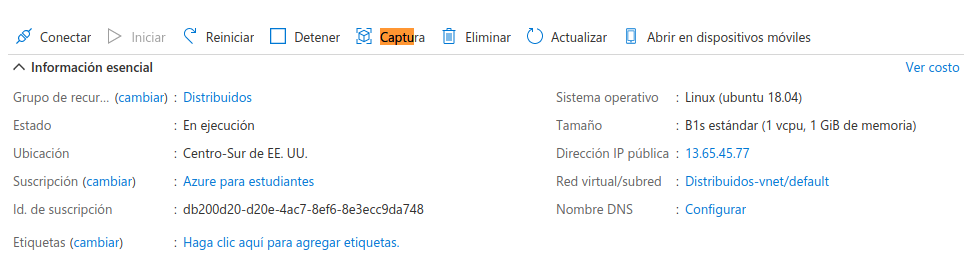
\includegraphics[scale=0.5]{imgs/3.png}\\
  \textit{Figura 3: Apartado de localización donde se encuentra la captura} \\
  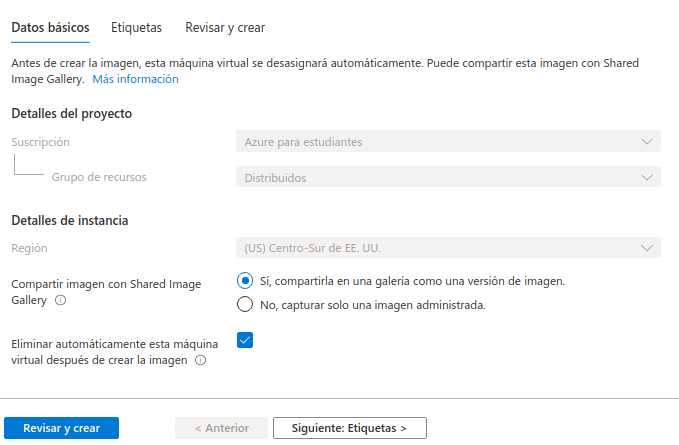
\includegraphics[scale=0.5]{imgs/4.png}\\
  \textit{Figura 4: Casilla seleccionada de eliminación de VM}\\
  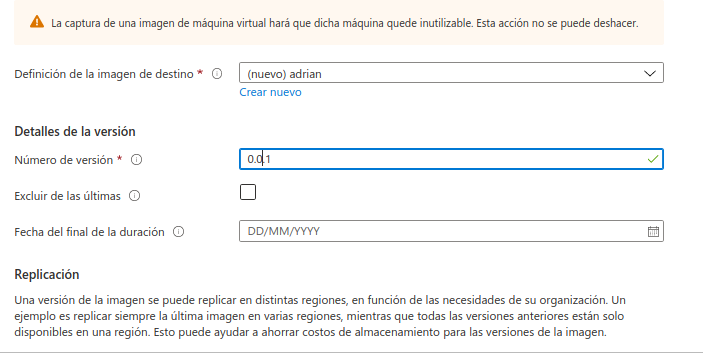
\includegraphics[scale=0.5]{imgs/5.png}\\
  \textit{Figura 5: Datos a llenar}\\
  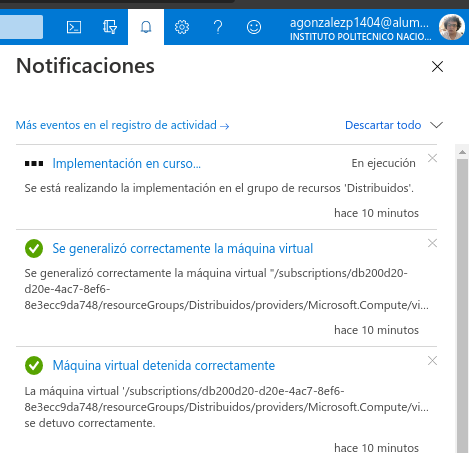
\includegraphics[scale=0.5]{imgs/6.png}\\
  \textit{Figura 6: En espera del termino del trabajo}\\
  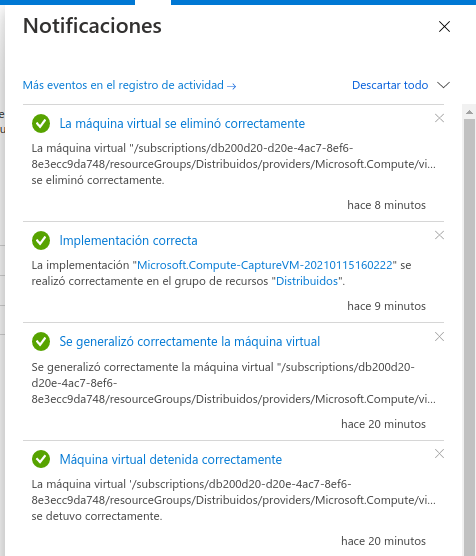
\includegraphics[scale=0.5]{imgs/7.png}\\
  \textit{Figura 7: Completes de trabajo y de eliminación de trabajo}
\end{center}
\subsection{Crear una máquina virtual a partir de la imagen creada}
Para finalizar iremos al menú de Azure en todos los recursos y seleccionaremos la imagen de la VM.
\begin{center}
  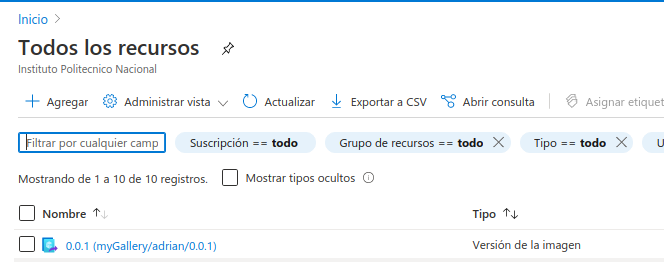
\includegraphics[scale=0.5]{imgs/8.png}\\
  \textit{Figura 8: Localización de la imagen, se procede a seleccionar}
\end{center}
Se seleccionara en crear imagen
\begin{center}
  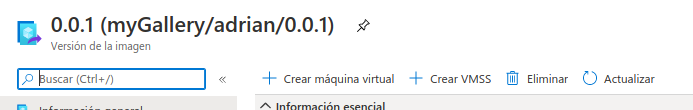
\includegraphics[scale=0.5]{imgs/9.png}\\
  \textit{Figura 9: Menú de imagen de vm se selecciona en crear vm}
\end{center}
Posteriormente llenaremos lo siguiente:
\begin{center}
  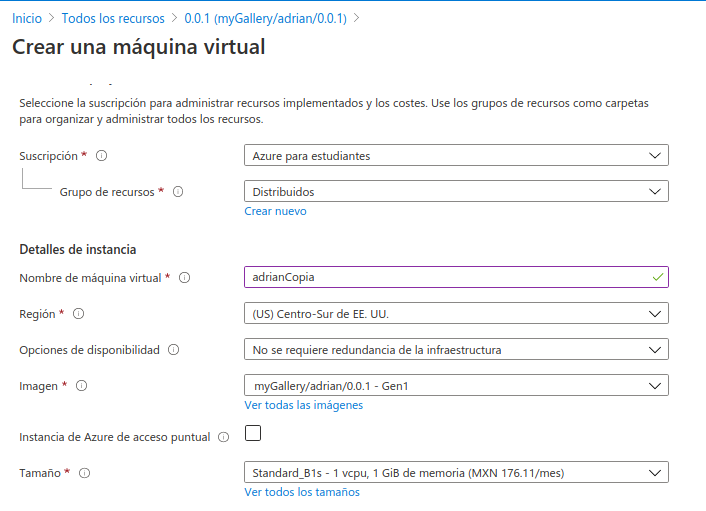
\includegraphics[scale=0.5]{imgs/10.png}\\
  \textit{Figura 10: Llenado de campos que utilizara la VM}\\
  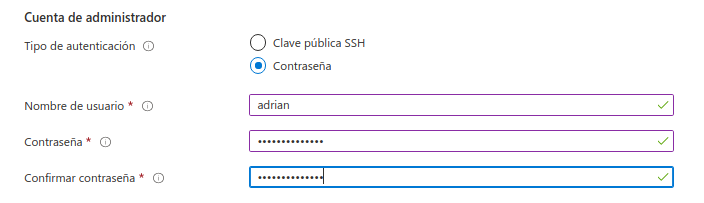
\includegraphics[scale=0.5]{imgs/11.png}\\
  \textit{Figura 11: Forma de inicio de sesión con contraseña}\\
  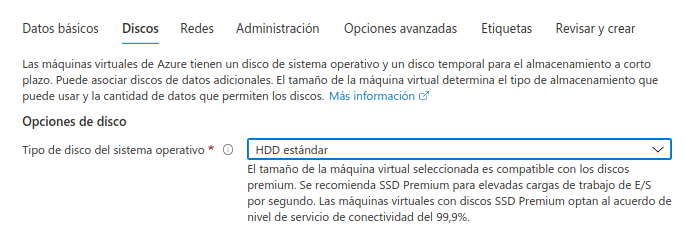
\includegraphics[scale=0.5]{imgs/12.png}\\
  \textit{Figura 12: Configuración de tipo de disco}\\
  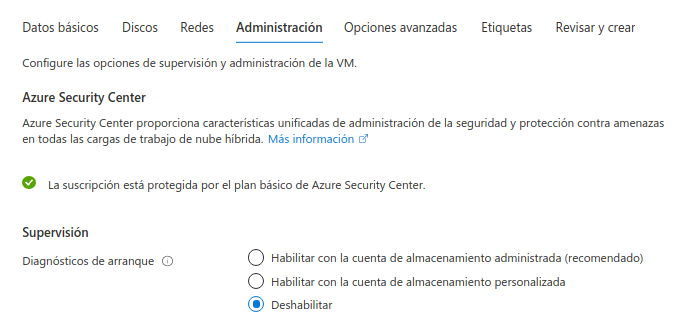
\includegraphics[scale=0.5]{imgs/13.png}\\
  \textit{Figura 13: Configuración administrativa}\\
  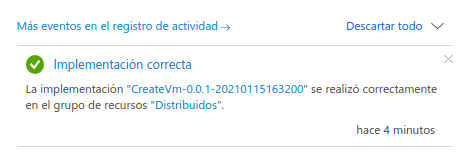
\includegraphics[scale=0.5]{imgs/14.png}\\
  \textit{Figura 14: Tarea finalizada}
\end{center}
Posteriormente a todo esto procederemos a crear la VM a partir de nuestra imagen y la veremos en el menú de vm's de azure
\begin{landscape}
  \begin{center}
    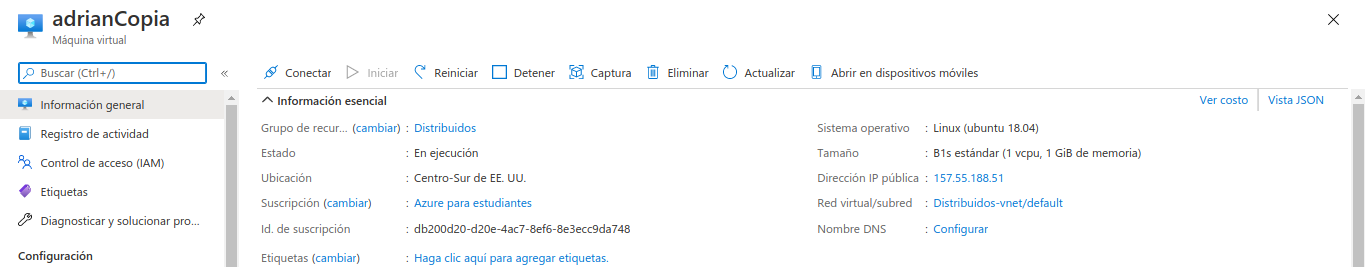
\includegraphics[scale=0.45]{imgs/15.png}\\
    \textit{Figura 15: Información de la VM a partir de la imagen}
  \end{center}
  \section{Conclusión}
  El poder crear snapshots o copias directas de una VM nos permite poder crear o pensar en que podemos generar copia de nuestras implementaciones antes de alguna desgracia la cual pueda como bien dicen \textit{tumbar} todo nuestro trabajo, pensando en que tendremos que realizar una vuelta atras antes de la tragedia, por ello este tipo de utilidades o de herramientas nos permite ahorrar mucho tiempo a la hora de replicar alguna maquina/servicio.
  \fillandplacepagenumber
\end{landscape}
\end{document}
